\section{Echo-state networks}

\mode<presentation>{
\begin{frame} 
    \begin{center} \huge
        \secname
    \end{center}
    \begin{center}
    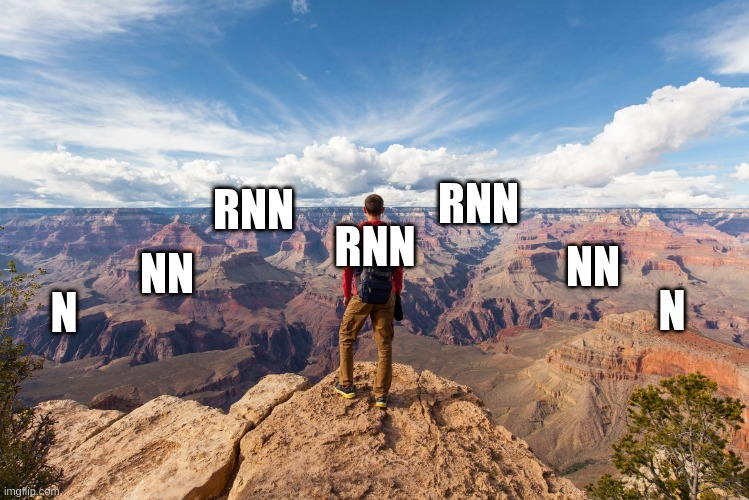
\includegraphics[width=0.3\textwidth]{img/meme_echo}
    \end{center}
    \begin{center}
    A solution to the vanishing gradient problem in RNNs
    \end{center}
\end{frame}
}

\definecolor{darkgreen}{rgb}{0,0.5,0}
\definecolor{darkyellow}{rgb}{0.5,0.5,0}
\definecolor{midgreen}{rgb}{0,0.75,0}

% ------------------------------------------------------------------------------
\begin{frame}\frametitle{Echo-state networks}
	\placeimage{13.75}{0.75}{img/rnn.pdf}{height=3cm}
		\iitem{system dynamics determine the input representation
			\vspace{1mm}
			\iitem{non-linear preprocessing step with memory}}
		\vspace{4mm}
		\iitem{address vanishing gradients by keeping $\vec W$ and $\vec U$ fixed
			\vspace{1mm}
			\iitem{output weights $\vec V$ can be trained by e.g.~linear regression}
			\vspace{-1mm}
			\iitem{hidden ``reservoir'' maintains inputs/errors over time}
			%\vspace{-2mm}
			%\iitem{hidden dynamics must be rich enough to bridge the gap}
		}
		\vspace{4mm}
		\iitem{system dynamics determine how fast inputs/errors are forgotten}
	\blfootnote{\hfill\citep[Section 10.8]{Jaeger04,Goodfellow16}}
\end{frame}

\subsection{Initialization of weight matrices}

% ------------------------------------------------------------------------------
\begin{frame}\frametitle{Echo-state networks: Careful weight initialization}
	\placeimage{13.75}{0.75}{img/rnn.pdf}{height=3cm}
		\iitem{eigenvalues $\lambda_i$ of the system's {\em Jacobian} $\vec J$}
			$$
				J_{ij}^{(t)} 
				\quad=\quad 
				%~ \smallfrac{\partial h_i^{(t)}}{\partial h_j^{(t-1)}}
				%~ \quad=\quad
				%~ f'\big(h_i^{(t)}\big) \cdot W_{ij}
				\smallfrac{\partial h_i^{(t)}}{\partial h_j^{(t-1)}}
				\quad=\quad
				 W_{ij} \, f'\big(h_j^{(t)}\big)
				\hspace{2cm}
			$$
            $$
                h_i^{(t)} = \smallsum{j=1}{H} W_{ij} \, f(h_j^{(t-1)})
            $$
		\vspace{2mm}
		\iitem{eigenvectors with $|\lambda_i| \approx 1$ 
				vanish/explode {\em very slowly}
			\vspace{1mm}
			\iitem{inputs/errors are maintained for a long time}}
		\vspace{6mm}
		\iitem{generate random $\vec W$, and $\vec U$ 
				where all $|\lambda_j| \approx r$
			\vspace{1mm}
			%~ \iitem{$f'(h_i^{(t)}) < 1$ \quad is a contraction $\quad\leadsto\quad$ $r > 1$}
			\iitem{$f'(h_j^{(t)}) < 1$ \quad is a contraction $\quad\leadsto\quad$ $r > 1$}
			\vspace{-1mm}
			\iitem{values between $r=1.2$ and $r=3$ are used in practice}
			\vspace{-2mm}
			%\iitem{$n$ hidden neurons can maintain
					%inputs/errors for up to $n$ time steps }
					}
	\blfootnote{\hfill\citep[Section 10.8]{Jaeger04,Goodfellow16}}
\end{frame}

